%& C:\Users\lizil\AppData\Roaming\TikzEdt\TikzEdt\023~1.0\TEMP_H~1
\begin{document}
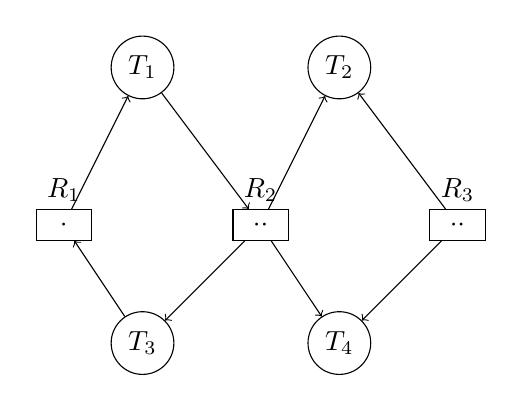
\begin{tikzpicture}
\tikzstyle{label} = [above,yshift=5pt];
\tikzstyle{res}=[minimum width=20pt,minimum height=5pt,draw];
\tikzstyle{pro}=[circle,draw];
\tikzstyle{alloc}=[->];
\node [res] (v1) at (-3,1) {$\cdot$};
\node [label] at (v1) {$R_1$};
\node [pro] (v2) at (-2,3) {$T_1$};

\node [pro] (v4) at (0.5,3) {$T_2$};
\node [pro] (v5) at (-2,-0.5) {$T_3$};
\node [res] (v3) at (-0.5,1) {$\cdot\cdot$};
\node [label] at (v3) {$R_2$};
\node [pro] (v6) at (0.5,-0.5) {$T_4$};
\draw [alloc] (v1) edge (v2);

\node (v7) [res] at (2,1) {$\cdot\cdot$};
\node [label] at (v7) {$R_3$};

\draw [alloc] (v2) edge (v3);
\draw [alloc] (v3) edge (v4);
\draw [alloc] (v7) edge (v4);
\draw [alloc] (v3) edge (v5);
\draw [alloc] (v5) edge (v1);
\draw [alloc] (v3) edge (v6);
\draw [alloc] (v7) edge (v6);

\usetikzlibrary{calc}
\pgftransformreset
\node[inner sep=0pt,outer sep=0pt,minimum size=0pt,line width=0pt,text width=0pt,text height=0pt] at (current bounding box) {};
%add border to avoid cropping by pdflibnet
\foreach \border in {0.1}
  \useasboundingbox (current bounding box.south west)+(-\border,-\border) rectangle (current bounding box.north east)+(\border,\border);
\newwrite\metadatafile
\immediate\openout\metadatafile=\jobname_BB.txt
\path
  let
    \p1=(current bounding box.south west),
    \p2=(current bounding box.north east)
  in
  node[inner sep=0pt,outer sep=0pt,minimum size=0pt,line width=0pt,text width=0pt,text height=0pt,draw=white] at (current bounding box) {
\immediate\write\metadatafile{\p1,\p2}
};
\immediate\closeout\metadatafile
\end{tikzpicture}

\end{document}
